\cotefile{93}
\scanpage{3}
\margin{G? = correction de Grothendieck}
\margin{Pour une version un brin plus complète :\par
Lecture Notes 476 (Anvers \uline{IV}) p 53--73\par
see also: Tate, ibidem p 33--52 et spécialement p 33--39}

\begin{center}
COURBES ELLIPTIQUES : FORMULAIRE

 d'après J. Tate

mis au goût du jour par P. Deligne
\end{center}

1.\quad \uline{Formules générales}.

Dans ce formulaire, on appellera courbe de genre 1 sur un schéma de base $S$ un morphisme propre et plat de présentation finie
\[
p:E\longrightarrow S,
\]
muni d'une section $e$ contenue dans l'ouvert de lissité, dont les fibres géométriques sont des courbes réduites irréductibles de genre \uline{ar}ithmétique 1. Les fibres géométriques de $p$ sont donc soit :
\margin{G?}

 a) une courbe elliptique, i.e. une courbe propre, lisse et connexe de genre 1,

 b) une droite projective dont on a identifié deux points distincts (cubique dans $P_2$ à point double ordinaire),

 c) une droite projective dont on a identifié deux points infiniment voisins (cubique dans $P_2$ à singularité cuspidale).

On dira dans le cas a) (resp. b), c)) que la fibre est de type elliptique (resp. multiplicatif, resp. additif).

Si $E$ est une courbe de genre 1 sur $S$, on définit un faisceau inversible $\omega$ sur $S$ par la formule
\[
\omega=e^*\Omega^1_{E/S}.
\]
La section $e$ est un diviseur de Cortier relatif de $E$ sur $S$ ;
\margin{2}
\scanpage{4}
\uline{Formules utiles}
\[
1728\Delta=c_4^3-c_6^2
\]
\[
j=\frac{c_4^3}{\Delta}=1728+c_6^2/\Delta
\]
\[
c_4\in H^0(\unsure{\overline{\Pi}|\overline{M}},\omega^4)\quad
c_6=H^0(\unsure{\overline{\Pi}|\overline{M}},\omega^6)\quad
\Delta=H^0(\unsure{\overline{\Pi}|\overline{M}},\omega^{12}
\]
\margin{car $\ne 2,3$.}
\[
\begin{aligned}
c_4=0&\Longleftrightarrow 6\text{ auto}\Longleftrightarrow j=0\\
c_6=0&\Longleftrightarrow 4\text{ auto}\Longleftrightarrow j=1728
\end{aligned}
\]
\[
h\in H^0(\unsure{\overline{\Pi}|\overline{M}},\omega^{\otimes\deleted{\unsure{12}}\inserted{p-1}})
\]
\[
\deg\omega=1/24
\]
\figure{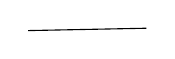
\begin{tikzpicture}\draw (0,0)--(1.5,.03);\end{tikzpicture}}
\[
\begin{aligned}
E=G_m/q^{\mathbb Z},\ \frac{du}{u}\quad\to\quad
c_4&=\left(\frac{du}{u}\right)^{\otimes4}\left(1+240\sum\sigma_3(n)q^n\right)\qquad(=E_4)\quad(Q)\\
c_6&=\left(\frac{du}{u}\right)^{\otimes6}\left(1\deleted{\unsure{+}}\inserted{-}504\sum\sigma_5(n)q^n\right)\qquad(=E_6)\quad(R)
\end{aligned}
\]
\figure{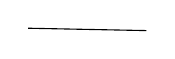
\begin{tikzpicture}\draw (0,0)--(1.5,-.03);\end{tikzpicture}}

Question : $h=\left(\dfrac{du}{u}\right)^{\otimes p-1}$ ? à l'$\infty$ --

\figure{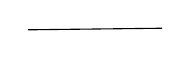
\begin{tikzpicture}\draw (0,0)--(1.7,.02);\end{tikzpicture}}
\[
y^2=x(x-1)(x-\lambda)\quad\longmapsto\quad j=2^8\frac{(1-\lambda(1-\lambda))^3}{(\lambda(1-\lambda))^2}
\]
\margin{[$\unsure{p^{\mathrm{ts}}}$ ordre 2 marqués]
\diagram{$\boxed{\begin{array}{l}
\lambda\\1-\lambda\\\lambda^{-1}\\1-\lambda^{-1}\\(1-\lambda)^{-1}\\\unsure{-}(1-\lambda^{-1})^{-1}
\end{array}}$}}
\figure{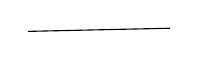
\begin{tikzpicture}\draw (0,0)--(1.8,.04);\end{tikzpicture}}
\uline{Hasse} : $(-1)^n\sum\binom{n}{i}^2\lambda^i$

ou $n=\dfrac{p-1}{2}$

\diagram{$\begin{array}{c@{\quad}cccc@{\quad}l}
p\equiv&1&5&7&11&(12)\\
\lambda=& &0&1728&\begin{array}{c}0\\1728\end{array}&\text{et }\dfrac{p-\unsure{\bullet}}{12}\text{ autres --}
\end{array}$}
\figure{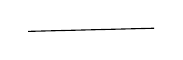
\begin{tikzpicture}\draw (0,0)--(1.6,.04);\end{tikzpicture}}
\margin{3}
\scanpage{5}
- \mspage{2} -

de plus, on vérifie fibre par fibre que
\[
R^1p_*\mathcal O(ne)=0\quad\text{pour}\quad n>0.
\]
Il en résulte, par Riemann-Roch, que pour $n>0$, le faisceau $p_*\mathcal O(ne)$ est localement libre de rang $n$, et que sa formation commute à tout changement de base. La suite exacte de cohomologie fournit de plus une suite exacte
\diagram{\begin{tikzcd}[column sep=small]
0\arrow[r]&p_*\mathcal O(ne)\arrow[r]&p_*\mathcal O((n+1)e)\arrow[r]&\omega^{\otimes-(n+1)}\arrow[r]&0
\end{tikzcd}\quad $(n>0)$.}
Par ailleurs, $\mathcal O(e)$ étant localement libre de rang 1, on vérifie fibre par fibre, compte tenu de (SGA 1 X 1.2), que
\diagram{\begin{tikzcd}
\mathcal O_S\arrow[r,"\sim"]&p_*\mathcal O_E\arrow[r,"\sim"]&p_*\mathcal O(e)
\end{tikzcd}.}
En d'autres termes, les $p_*\mathcal O(me)$ pour $1\leq m\leq n$ définissent une filtration de $p_*\mathcal O(ne)$, de gradué associé
\[
(1.1)\qquad \mathrm{Gr}\ p_*\mathcal O(ne)=\sum_{\substack{i=0\\i\ne1}}^n\omega^{\otimes-i}.
\]

Le morphisme $p$ est d'intersection complète relative ; il en résulte que $Rp^!\mathcal O_S\in D^+(E)$ \inserted{\unsure{$\rho$}} a un seul groupe de cohomologie non nulle, $R^1p^!\mathcal O_S$, et que ce dernier est un faisceau inversible sur $E$ ; on l'appelle le faisceau des différentielles régulières sur $E$ et on le désigne par $\Omega^{\mathrm{reg}}_{E/S}$. Là où $p$ est lisse, on a $\Omega^{\mathrm{reg}}_{E/S}=\Omega^1_{E/S}$. La dualité montre que $R^1p_*\Omega^{\mathrm{reg}}_{E/S}$ est isomorphe à $\mathcal O$, $p_*\Omega^{\unsure{\mathrm{rog}|\mathrm{reg}}}_{E/S}$ est donc\inserted{\unsure{$\rho$}} localement libre, de formation compatible à tout changement de base et, raisonnant fibre par fibre, on en déduit que
\margin{\uline{réf}}
\margin{\uline{réf}}
\margin{4}
\scanpage{6}
- \mspage{3} -
\diagram{\begin{tikzcd}
p_*\Omega^{\mathrm{reg}}_{E/S}\arrow[r,"\sim"]&\unsure{o^*|e^*}\Omega^1_{E/S}=\omega
\end{tikzcd},}
et que pour la flèche adjointe à la flèche inverse
\diagram{\begin{tikzcd}
p^*\omega\arrow[r,"\sim"]&\Omega^{\mathrm{reg}}_{E/S}
\end{tikzcd}.}
Les sections de $\Omega^{\mathrm{reg}}_{E/S}$ ainsi associées aux sections de $\omega$ s'appellent les différentielles invariantes.

Soit $\pi$ une section inversible de $\omega$ ; il existe, localement pour la topologie de Zariski, une base $(y,x,1)$ de $p_*\mathcal O(3e)$ telle que l'image de $y$ dans $\omega^{\otimes-3}$ soit $-\pi^{\otimes-3}$, que $x$ appartienne à $p_*\mathcal O(2e)$, et que son image dans $\omega^{\otimes-2}$ soit $\pi^{\inserted{\otimes}-2}$. Si $\pi'$ est une autre section inversible de $\omega$, les bases correspondantes s'écrivent toutes, sous forme implicite (pour $r,s,t$ convenables)
\margin{G?}
\[
(1.2)\qquad\left\{\begin{aligned}
x&=u^2x'+r\\
y&=u^3y'+su^2x'+t\\
\pi'&=u\pi
\end{aligned}\right.\qquad .
\]
Le faisceau $\mathcal O(3e)$ est très ample et $(x,y,1)$ sont les coordonnées projectives d'un plongement de $E$ dans $P_2/S$.

La courbe image vérifiera une équation
\[
(1.3)\qquad y^2+a_1xy+a_3y=x^3+a_2x^2+a_4x+a_6.
\]
Pour vérifier l'existence et l'unicité de cette équation, on
\margin{5}
\scanpage{7}
- \mspage{4} -

utilise (1.1), en regardant les deux membres de (1.3) comme des sections de $p_*\mathcal O(6e)$ : en effet, $y^2-x^3$ est dans $p_*\mathcal O(5e)$, $xy$ dans $p_*\mathcal O(5e)$, $x^2$ dans $p_*\mathcal O(4e)$, $y$ dans $p_*\mathcal O(3e)$, $x$ dans $p_*\mathcal O(2e)$ et $1$ dans $p_*\mathcal O$.

Si on pose
\[
F(x,y)=y^2+a_1xy+a_3y-x^3-a_2x^2-a_4x-a_6
\]
la forme différentielle invariante définie par $\pi$ s'écrit
\[
\pi=dx/F_y=-dy/F_x\qquad\text{soit}
\]
\[
\pi=\frac{dx}{2y+a_1x+a_3}=\frac{dy}{3x^2+2a_2x+a_4-a_1y}.
\]
Réciproquement toute équation (1.3) est l'équation non homogène d'une courbe de genre 1 plongée comme une cubique dans $P_2$ et présentant un point d'inflexion en $(0,1,0)$ avec la droite de l'infini pour tangente d'inflexion.

On pose alors
\[
(1.4)\qquad b_2=a_1^2+4a_2\qquad b_4=a_1a_3+2a_4\qquad b_6=a_3^2+4a_6
\]
\[
-b_8=a_1a_3a_4+a_4^2-a_1^2a_6-a_2a_3^2-4a_2a_6
\]
\[
d_6=b_2b_4-18b_6\qquad d_8=b_2^2b_4-2^4\,3\,b_4^2+2\,3^2\,b_2b_6
\]
On a
\[
-4b_8=b_4^2-b_2b_6
\]
\[
12d_6=c_6+b_2c_4\qquad -12d_8=c_4^2+b_2c_6
\]
\margin{6}
\scanpage{8}
- \mspage{5} -
\[
(1.5)\qquad c_4=b_2^2-24b_4\qquad -c_6=b_2^3-36b_2b_4+216b_6
\]
\[
\begin{aligned}
\Delta&=-b_2^2b_8-8b_4^3-27b_6^2+9b_2b_4b_6\\
&=b_4^3-27b_6^2+b_8(36b_4-b_2^2).
\end{aligned}
\]
Soient maintenant $(x',y',\pi')$ reliés à $(x,y,\pi)$ par (1.2). On aura :
\[
\begin{aligned}
(1.6)\qquad ua'_1&=a_1+2s\\
u^2a'_2&=a_2-sa_1+3r-s^2\\
u^3a'_3&=a_3+ra_1+2t=F_t(r,t)\\
u^4a'_4&=a_4-sa_3+2a_2r-(t+rs)'a_1+3r^2-2st=-F(r,t)-sF_t(r,t)\\
u^6a'_6&=a_6+ra_4+r^2a_2+r^3-ta_3-t^2-rta_1=-F(r,t)
\end{aligned}
\]
\[
\begin{aligned}
(1.7)\qquad u^2b'_2&=b_2+12r\\
u^4b'_4&=b_4+rb_2+6r^2\qquad\text{(équ. de discr. }c_4\text{)}\\
u^6b'_6&=b_6+2rb_4+r^2b_2+4r^3\qquad\text{(équ. de discr. }16\Delta\text{)}\\
u^8b'_8&=b_8+3rb_6+3r^2b_4+r^3b_2+3r^4
\end{aligned}
\]
\[
u^6d'_6=d_6+c_4r\qquad u^8d'_8=d_8-c_6r
\]
\margin{7}
\scanpage{9}
- \mspage{6} -
\[
(1.8)\qquad u^4c'_4=c_4\qquad u^6c'_6=c_6\qquad u^{12}\Delta'=\Delta.
\]
Les formules (1.8) expriment que la section $c_4\pi^{\otimes4}$ (resp. $c_6\pi^{\otimes6}$, \unsure{rosp.|resp.} $\Delta\pi^{\otimes12}$) du fibré $\omega^{\otimes4}$ (resp. $\omega^{\otimes6}$, $\omega^{\unsure{\circ|\otimes}12}$) ne dépend pas du choix arbitraire de $\pi$, $x$ et $y$.

2.\quad \uline{Cas où 2 et 3 sont inversibles}.

Lorsque 2 et 3 sont inversibles, on peut d'une et d'une seule façon choisir $x$ et $y$ ($\pi$ étant donné) de sorte que dans l'équation (1.3.) on ait $a_1=a_2=a_3=0$. On a alors
\[
(2.1)\qquad y^2=x^3+a_4x+a_6,\ \text{avec}\quad\pi=dx/2y,
\]
\[
(2.2)\qquad c_4=-2^4\cdot3a_4,\quad c_6=-2^5\cdot3^3a_6,\quad\Delta=2^4(-4a_4^3-27a_6^2).
\]
Posant $Y=2y$, $X=x$, on retombe sur la forme de Weierstrass
\[
(2.3)\qquad Y^2=4X^3-g_2X-g_3,\quad\text{avec}\quad\pi=dX/Y,\quad\text{et}
\]
\[
(2.4)\qquad g_2=-4a_4=\frac1{12}c_4\qquad g_3=-4a_6=\frac1{216}c_6
\]
\[
\Delta=g_2^3-27g_3^2.
\]
\uline{Proposition} 2.5.\quad \uline{Au dessus de} $\mathrm{Spec}(\mathbb Z[2^{-1},3^{-1}]$, \uline{il existe un schéma de modules pour les courbes de genre un munies d'une forme différentielle invariante inversible}. \uline{\unsure{C;|Ce} schéma est}
\[
\mathrm{Spec}(\mathbb Z[2^{-1},3^{-1}][g_2,g_3],
\]
\margin{8}
\scanpage{10}
- \mspage{7} -
\uline{avec pour courbe universelle} (\uline{en coordonnées non homogènes}) \inserted{\unsure{$\rho$}}
\margin{section $e$}
\[
Y^2=4X^3-g_2X-g_3
\]
\uline{et pour différentielle invariante} $\pi=dX/Y$.

De plus, lorsque 2 et 3 sont inversibles, la donnée d'une forme différentielle invariante suffit à rigidifier une courbe de genre 1.

Il résulte aussitôt de (2.2) qu'on a
\[
(2.6)\qquad c_4^3-c_6^2=1728\Delta
\]
et cette formule, se réduisant à une identité algébrique, est valable en toute caractéristique.

3. -\quad \uline{Cas où} 2 \uline{et} $c_4$ \uline{sont inversibles}.

Supposons que $E$ soit une courbe de genre un sur une base $S$ où 2 soit inversible. La forme différentielle invariante $\pi$ étant donnée, on peut choisir $x$ et $y$ tels que dans (1.3) on ait $a_1=a_3=0$. Les changements de coordonnées respectant cette condition s'obtiennent en faisant $u=1$, $s=t=0$ dans (1.2).

On a donc
\[
(3.1)\qquad y^2=x^3+a_2x^2+a_4x+a_6
\]
\[
b_2=4a_2\qquad b_4=2a_4\qquad b_6=4a_6\qquad d_6=8(a_2a_4-9a_6)
\]
\[
(3.2)\qquad c_4=2^4(a_2^2-3a_4)\qquad -c_6=2^6a_2^3-2^5\,3^2\,a_2a_4+2^5\,3^3\,a_6\quad\text{et}
\]
\[
\Delta=2^4\delta,
\]
\margin{9}
\scanpage{11}
- \mspage{8} -

où $\delta$ est le discriminant du second membre de (3.1). Le discriminant $\delta$ étant invariant par translation, il suffit de vérifier cette identité algébrique pour 3 inversible et $a_2=0$.

Lorsque $c_4$ est inversible, un et un seul choix de $x$ et $y$ donne $d_6=0$, i.e. $a_2a_4-9a_6=0$. On a, lorsque cette condition est remplie,
\[
(3.3)\qquad -c_6=2^6(a_2^3-3^3a_6)\qquad\Delta=2^6(-a_2^3a_6-a_4^3+2\cdot3^3a_6^2)
\]
et
\[
\begin{aligned}
(3.4)\qquad a_2c_4&=-2^{-2}c_6\\
a_4c_4^2&=-2^2\,3^2\,\Delta\\
a_6c_4^3&=c_6\Delta.
\end{aligned}
\]
Il suffit de vérifier ces identités en caractéristique 0, auquel cas la troisième est le produit des deux premières, puisque $d_6=0$.

\uline{Proposition} 3.5.\quad \uline{Au dessus de} $\mathrm{Spec}(\mathbb Z[2^{-1}])$, \uline{il existe un schéma de module pour les courbes de genre un munies d'une forme différentielle invariante inversible et telles que} $c_4$ \uline{soit inversible. Ce schéma est}
\[
\mathrm{Spec}(\mathbb Z[2^{-1}][a_2,a_4,a_6,(a_2^2-3a_4)^{-1}]/(a_2a_4-9a_6))
\]
\uline{avec pour courbe universelle} (\uline{en coordonnées non homogène}) \inserted{\unsure{$\rho$}}
\margin{section $e$}
\[
y^2=x^3+a_2x^2+a_4x+a_6
\]
\margin{10}
\scanpage{12}
- \mspage{9} -
\uline{et pour différentielle invariante} $\pi=dx/2y$.

De plus, sous ces hypothèses, la donnée d'une forme différentielle invariante suffit à rigidifier une courbe.

4.\quad \uline{Cas où} 2 \uline{est nilpotent et} $c_4$ \uline{inversible}.

Lorsque $2=0$, la forme différentielle ne suffit plus jamais à rigidifier une courbe de genre un. Lorsque $c_4$ est inversible et 2 nilpotent, donc $a_1$ inversible, en changeant le choix de $\pi,x,y$ on peut trouver une équation
\[
(4.1)\qquad y^2+xy=x^3+a_2x^2+a_6\qquad\pi=\frac{dx}{x+2y}.
\]
Les autres choix de $x$ et $y$ donnant lieu à une telle équation s'obtiennent en faisant, dans (1.2)
\[
(4.2)\qquad r=t=0\qquad u=1+2s
\]
et on aura
\[
\begin{aligned}
(4.3)\qquad u^2a'_2&=a_2-s-s^2\\
u^6a'_6&=a_6
\end{aligned}
\]
et \uline{modulo 2}
\[
(4.4)\qquad c_4=1\qquad c_6=1\qquad\Delta=a_6.
\]

5.\quad \uline{Cas où} $c_4=0$, $p=2$ \uline{ou} $p=3$

a) $p=3$

En caractéristique 3, lorsque l'équation est mise sour forme
\margin{11}
\scanpage{13}
- \mspage{10} -

(3.1), $c_4=0$ si et seulement si $a_2^2=0$. Supposons qu'on ait même $a_2=0$
\[
(5.1)\qquad y^2=x^3+a_4x+a_6\qquad\pi=a_4^{-1}dy=dx/2y
\]
\[
c_4=c_6=0\qquad\Delta=-a_4^3.
\]
Les autres systèmes $(\pi,x,y)$ donnant une équation de cette forme s'obtiennent en faisant $s=t=0$ dans (1.2) et
\[
\begin{aligned}
u^4a'_4&=a_4\\
(5.2)\qquad&\\
u^6a'_6&=a_6+ra_4+r^3.
\end{aligned}
\]
b) $p=2$

En caractéristique 2, on a $c_4=a_1^4$. Supposons qu'on ait $a_1=0$ ; $\pi$ étant donnée, on peut alors choisir $x$ et $y$ tels que (1.3) soit
\[
(5.3)\qquad y^2+a_3y=x^3+a_4x+a_6\qquad\pi=\frac{dx}{a_3}=dy/{}_{x^2+a_4}:
\]
\[
b_2=b_4=0\qquad b_6=a_3^2\qquad b_8=a_4^2\qquad\Delta=a_3^4\qquad c_4=c_6=0.
\]
Les autres systèmes $(\pi,x,y)$ donnant une équation de cette forme s'obtiennent en faisant $r=s^2$ dans (1.2) et
\[
\begin{aligned}
u^3\unsure{a'_3|e'_3}&=a_3\\
(5.4)\qquad u^4a'_4&=a_4+sa_3+s^4\\
u^6a'_6&=a_6+s^2a_4+ta_3+s^6+t^2.
\end{aligned}
\]
\margin{12}
\scanpage{14}
- \mspage{11} -
6.\quad \uline{Applications}.

\uline{Proposition} 6.1.\quad \uline{Si} $E$ \uline{est une courbe de genre un sur un corps algébriquement clos}, $E$ \uline{est de type elliptique} (\uline{resp. multiplicatif}, \uline{resp. additif}) \uline{si et seulement si} $\Delta\ne0$ (\uline{resp.} $\Delta=0$ et $c_4\ne0$, \uline{resp.} $\Delta=c_4=0$).

a) Lorsque la caractéristique $p\ne2$, la première assertion résulte de la troisième formule (3.2). Lorsque $p=2$ et $c_4\ne0$, on vérifie aussitôt que la différentielle de (4.1) ne s'annule qu'en $(0,0)$, et $\Delta$ est elliptique si et seulement si $\Delta=a_6\ne0$. Pour $p=2$ et $c_4=0$, on raisonne de même sur (6.2).

b) Lorsque $p\ne2$, il résulte de (3.2) que $\Delta=c_4=0$ si et seulement si le deuxième membre de (3.1) a toutes ses racines égales, ce qui caractérise le cas additif.

c) Lorsque $p=2$, $\Delta=0$, $c_4\ne0$, la partie principale de (4.1) en $(0,0)$ est $y^2+xy+a_2x^2=0$, ce qui correspond à un point double à tangentes distinctes.

d) Lorsque $p=2$, $\Delta=0$, $c_4=0$, la partie principale de (6.2) en $(0,0)$ est $y^2+a_4x+a_6=0$, ce qui correspond à une singularité cuspidale.

Soit alors $E$ une courbe de genre un sur une base $S$, sans fibre de type additif. Puisque $\Delta$ et $c_4$ ne sont jamais simultanément nuls, et sont respectivement des sections de $\omega^{\otimes12}$ et $\omega^{\otimes4}$, on définit une section $j$ de $P_1/S$ par la formule
\margin{13}
\scanpage{15}
- \mspage{12} -
\[
(6.2)\qquad j=c_4^3/\Delta=1728+c_6^2/\Delta.
\]
\uline{Proposition} 6.3.\quad \uline{Soient} $E$ \uline{et} $E'$ \uline{deux courbes de genre un sur} $S$, \uline{sans fibre additive}.

(I) $\uline{\mathrm{Isom}}_{\inserted{S}}(E,E')$ \uline{est représentable, fini et non ramifié sur} $S$

(II) \uline{si} $j_E=j_F$, \uline{la projection de} $\uline{\mathrm{Isom}}_{\inserted{S}}(E,E')$ \uline{sur} $S$ \uline{est surjective}

(III) \uline{si} $j_E=j_F$ \uline{ne prend pas les valeurs} 0 \uline{et} 1728, $\uline{\mathrm{Isom}}_{\inserted{S}}(E,E')$ \uline{est un revêtement étale de rang} 2 \uline{de} $S$.

Donnons-nous $E$ et $E'$ par des équations (1.3) et (1.3)'. Se donner un isomorphisme entre $E$ et $E'$ revient à se donner $u,r,s$ et $t$, vérifiant les équations (1.6), donc aussi (1.7) et (1.8), $u$ devant de plus être inversible. Par hypothèse, localement sur $S$, $c_4$ ou $\Delta$ est inversible (6.1), et de même $c'_4$ ou $\Delta'$ l'est. Localement sur $S$, les équations (1.8) sont donc des équations de dépendance intégrale pour $u$ et $u^{-1}$, les équations $(1.7)_6$ ou $(1.7)_8$ des équations de dépendance intégrale pour $r$ et enfin $(1.6)_6$ (resp. $(1.6)_2$) est une équation de dépendance intégrale pour $t$ (resp. $s$). Ceci prouve que $\uline{\mathrm{Isom}}(E,E')$ est représentable par un schéma affine fini sur $S$ ; il est même non ramifié car les courbes considérées n'ont pas d'automorphismes infinitésimaux (respectant l'origine).

Lorsque 2 est inversible sur $S$, l'assertion (III) résulte de l'énoncé plus précis.

\uline{Proposition} 6.4.\quad \uline{Soient} $E$ \uline{et} $E'$ \uline{deux courbes de genre un sur} $S$,
\margin{14}
\scanpage{16}
- \mspage{13} -
\uline{sans fibre additive}, \uline{munies de formes différentielles invariantes} $\pi$ \uline{et} $\pi'$, \uline{et de même invariant modulaire}. \uline{On suppose que} 2, $c_4$ \uline{et} $c_6$ \uline{sont inversibles}, \uline{i.e.} \uline{que} $2^{-1}$, $1/j$ et $1/(j-1728)$ \uline{sont des sections de} $S$. \uline{Alors}, \uline{le schéma} $\uline{\mathrm{Isom}}(E,F)$ \uline{s'identifie au schéma défini par l'équation}
\[
\lambda^2=c_4c'_6/c_6c'_4.
\]
En vertu de (3.6), se donner $(E,\pi)$ revient à se donner $a_2$, $a_4$ et $a_6$ vérifiant $a_2a_4-9a_6=0$, et un isomorphisme de $E$ sur $E'$ est décrit par $\lambda$ tel que $(E\ \pi)$ soit isomorphe à $(E',\lambda\pi')$, i.e. par $\lambda$ vérifiant
\[
(6.4.1)\qquad a'_2=\lambda^2a_2\qquad a'_4=\lambda^4a_4\qquad a'_6=\lambda^6a_6.
\]
Par hypothèse, $j=j'$, de sorte que $(c_4^3,c_6^2,\Delta)$ est proportionnel à $({c'_4}^3,{c'_6}^2,\Delta')$, et que $\mu=c_4c'_6/{}_{c_6c'_4}$ vérifie
\[
(6.4.2)\qquad c'_4=\mu^2c_4\qquad c'_6=\mu^3c_6\qquad\Delta'=\mu^6\Delta.
\]
En vertu de (3.4), on a alors
\[
a'_2=\mu a_2\qquad a'_4=\mu^2a_4\qquad a'_6=\mu^3a_6.
\]
\margin{\figure{\begin{tikzpicture}\draw (0,0)--(.35,-.015);\end{tikzpicture}}}
De plus, d'après (3.4) encore, localement, soit $a_2$, soit $a_4$ et $a_6$ sont inversibles, de sorte que (6.4.1) équivaut à $\lambda^2=\mu$.

Pour prouver (III) en général, on peut se ramener à supposer $S$ noethérien, et supposer soit 2 inversible (cas traité en (6.4)), soit
\margin{15}
\scanpage{17}
- \mspage{14} -

2 nilpotent, ce qui permet de mettre la courbe sous la forme (4.1)
\[
y^2+xy=x^3+a_2x+a_6
\]
et un isomorphisme d'une telle courbe sur une autre est décrit par $s$ vérifiant (4.3) pour $u=1+2s$. Lorsque $j=j'$, la première de ces équations
\[
(1+2s)^2a'_2=a_2-s-s^2
\]
définit un revêtement étale de degré deux, et elle implique la seconde ; pour le voir, on se ramène à supposer $a_2=a'_2$ et on remarque que d'après (4.4)
\[
1/j=a_6+2R(a_2,a_6)
\]
pour une fraction rationnelle $R$.

Pour vérifier (II) dans les cas non couverts par (III), on peut supposer que $S$ est le spectre d'un corps algébriquement clos et que $c_4=0$ ou $c_6=0$, i.e. que $j=0$ ou $j=1728$. Soit $p$ la caractéristique du corps,

a) $p\ne2,3$ : on met la courbe sous la forme (2.1) ; si $c_4=0$ (resp. $c_6=0$) on aura $a_4=0$ (resp. $a_6=0$) et on peut par homothétie transformer la courbe en la courbe type
\[
(6.5)\qquad y^2=x^3+1\qquad\text{(si }c_4=0\text{)}
\]
\[
(6.6)\qquad y^2=x^3-x\qquad\text{(si }c_6=0\text{)}
\]
b) $p=3$ : on met la courbe sour la forme (6.1) ; résolvant (6.2) pour $a'_4=1$ et $a'_6=0$, on met la courbe sous la forme type
\margin{16}
\scanpage{18}
\uline{Question connexe} : soit $E$ ell sur $k$ parfait.
\[
M^\wedge=\text{sch formel mod de }E\ (\text{sur }W(k))
\]
\diagram{\begin{tikzcd}[column sep=large]
\boxed{\mathrm{Spec}\ W(k)[j]^\wedge\sim M^\wedge/\mathrm{Aut}(E)} \arrow[r] & \text{étude }\unsure{\infty^{\mathrm{ale}}|\mathrm{locale}}\text{ à faire de }j.
\end{tikzcd}}

\diagram{\begin{array}{llll}
a)&j=0,\ p\ne2,3:&j\sim t^3&t\ \text{paramètre régulier relatif}\\
b)&j=12^3,\ p\ne2,3\unsure{:}&j\sim t^2&\text{''}\\
c)&\uline{j=0,\ p=3}:&\text{groupe }6\ \text{éléments}&-\\
d)&\uline{j=0,\ p=2}:&\text{''}\quad12\quad\text{''}&-
\end{array}}
\margin{\[
\begin{aligned}
\unsure{\parallel|\mathrm{II}}&=\mathrm{car}\ 3:\quad6\mid v(j)\\
&=\mathrm{car}\ 2:\quad12\mid v(j)
\end{aligned}
\]}
\margin{\unsure{$\rho$} ? semi direct de $\mathbb Z/3$ par $\{\pm1\ \pm i\ \pm j\ \pm\unsure{h|k}\}$ ou $\mathbb Z/3$ agit par $(i,j,k)$\quad--}
\margin{17}
\scanpage{19}
- \mspage{15} -
\[
(6.7)\qquad y^2=x^3-x\qquad(\text{si }c_4=c_6=0)
\]
c) $p=2$ : ici, on met la courbe sour la forme (6.3) et on résoud (6.4) avec $a_3=1$, $a_4=a_6=0$ pour obtenir la forme type
\[
(6.8)\qquad y^2+y=x^3\qquad(\text{si }c_4=c_6=0).
\]
Pour compléter le tableau, reste à décrire les automorphismes des courbes elliptiques.

\uline{Proposition} 6.9.\quad\uline{Soit} $E$ \uline{une courbe de genre un sur une base} $S$, \uline{sans fibre additive}

(I) \uline{Si} $c_4$ et $c_6$ \uline{sont inversibles, les seuls automorphismes de} $E$ \uline{sont l'identité et la symétrie}.
\margin{[vrai seulement en faisceautisant !]}

(II) \uline{Si} 2 et 3 \uline{sont inversibles, l'application canonique}
\[
(6.6.)\qquad\diagram{\begin{tikzcd}\uline{\mathrm{Aut}}(E)\arrow[r]&G_m\end{tikzcd}}
\]
\uline{donnée par l'action sur les différentielles invariantes, est une immersion fermée}.

(III) \uline{Si} 2 \uline{et} 3 \uline{sont inversibles}, \uline{et} $c_4=0$ (resp. $c_6=0$) \uline{l'image de} (6.6) \uline{est} $\mu_6$ (resp. $\mu_4$).

\uline{Supposons maintenant que} $S$ \uline{soit le spectre d'un corps}

(IV) \uline{Si} $3=c_4=c_6=0$, $\mathrm{Aut}(E)$ \uline{est géométriquement \unsure{isomorphe} au produit semi-direct} (\uline{non commutatif}) \uline{de} $\mathbb Z/(4)$ \uline{par} $\mathbb Z/(3)$, \uline{et l'image de} (6.6) \uline{est} $\mu_4$.

(V) \uline{Si} $2=c_4=c_6=0$, $\mathrm{Aut}(E)$ \uline{est géométriquement d'ordre} 24, \uline{et l'image de} (6.6) \uline{est} $\mu_3$.
\margin{\unsure{$\rho$}}
\margin{18}
\scanpage{20}
- \mspage{16} -
\uline{Preuve} : (I) D'après (6.3), il n'y a en effet pas plus de deux automorphismes.

(II) et (III)\quad Lorsque les courbes sont mises sous la forme (2.1), il résulte de (2.5) que les automorphismes sont décrits parleur action sur $\pi$ et que $\lambda\in G_m$ défini un automorphisme si et seulement si
\[
c_4=\lambda^4c_4\qquad\text{et}\qquad c_6=\lambda^6c_6\qquad,
\]
d'où les assertions.

(IV)\quad Si la courbe est mise sous forme (6.1), les automorphismes sont donnés par (1.2) : $x'\leadsto x$, pour $s=t=0$ et
\[
\left\{\begin{aligned}
u^4&=1\\
r^3+ra_4+a_6(1-u^2)&=0
\end{aligned}\right.
\]
et la loi de composition par
\[
(u',r')\quad(u,r)=(u\,u',\ u'^2r+r')
\]
Lorsque la courbe est mise sous forme (6.7), ces équations se réduisent à $u\in\mu_4$ et $r\in\mathrm F_3$.

(V)\quad Si la courbe est mise sous forme (6.3), les automorphismes sont donnés par (1.2) : $x'\leadsto x$, pour $r=s^2$ et
\[
\left\{\begin{aligned}
u^3&=1\\
s^4+sa_3+a_4(1-u)&=0\\
t^2+ta_3+s^6+s^2a_4&=0
\end{aligned}\right.
\]
\margin{19}
\scanpage{21}
\uline{Cor} : pour $\unsure{S|E}$ plat sur $\mathbb Z$,\qquad $\Gamma(S,\mathcal O_S)[\cdots]$
\margin{[ou \unsure{seul$^{\uline{\mathrm{mt}}}$|seul$^{\uline{\mathrm{nt}}}$} 2 et 3 non div. de 0]}
\margin{20}
\scanpage{22}
- \mspage{17} -
et la loi de composition par
\[
(u',s',t')\circ(u,s,t)=(u\,u',u's+t',u'^3t+t'+u'^2rs').
\]
Lorsque la courbe est mise sous forme (6.8), ces équations se réduisent à
\[
u\in\mu_3\quad s\in\mathbb F_4\qquad t^2+t=s^3\quad(=0\text{ ou }1\text{ selon que }s=0\text{ ou }s\ne0).
\]

7.\quad\uline{Anneau des formes modulaires entières}.

On appelle forme modulaire entière de poids $n$ une loi qui à chaque courbe de genre un sur une base $S$ associe une section de $\omega^{\otimes n}$, et ce de façon compatible au changement de base. Il reviendrait au même de se limiter aux courbes sans fibres additives.

\uline{Proposition} 7.1.\quad\uline{L'anneau des formes modulaires entières est engendré sur} $\mathbb Z$ \uline{par} $c_4$, $c_6$ \uline{et} $\Delta$ \uline{soumis à la seule relation}
\[
(7.2.)\qquad c_4^3-c_6^2=1728\,\Delta\quad.
\]
Appliquant la définition à la courbe (1.3), on voit qu'une forme modulaire entière de poids $n$ s'exprime comme polynôme de poids $n$ en les $a_i$. Pour 2 et 3 inversibles, il résulte de 2.5 que ces formes sont les polynômes en $c_4$ et $c_6$, et en particulier que $c_4$, $c_6$ et $\Delta$ ne satisfont pas d'autres relations que (7.2). Reste à prouver que si un polynôme en $c_4$, $c_6$ et $\Delta$ est identiquement nul en caractéristique 2 (resp. 3), alors il est divisible par 2 (resp.3) dans $\mathbb Z[c_4,c_6,\Delta]/c_4^3-c_6^2-1728\,\Delta$, ce qui signifie
\margin{G?}
\margin{21}
\scanpage{23}
$a_1$ et $\pm b_2$ sont les invariants de Hasse Witt.
\margin{22}
\scanpage{24}
- \mspage{18} -
qu'il est divisible par $c_4^3-c_6^2$ dans $\mathbb Z/(2)[c_4,c_6,\Delta]$ (resp. $\mathbb Z/(3)[c_4,c_6,\Delta]$). Cela résulte de la structure de l'anneau des formes modulaires de caractéristique 2 (resp. 3).

\uline{Proposition} 7.2.\quad(I) \uline{L'anneau des formes modulaires de caractéristique} 2 \uline{est} $\mathbb Z/(2)[a_1,\Delta]$, \uline{et} $c_4=a_1^4$, $c_6=a_1^6$

(II) \uline{L'anneau des formes modulaires de caractéristique} 3 \uline{est} $\mathbb Z/(3)[b_2,\Delta]$, et $c_4=b_2^2$, $c_6=-b_2^3$.

Tout d'abord, il résulte de $(1.6)_1$ et $(1.7)_2$ que $a_1$ (resp. $b_2$) est une forme modulaire de caractéristique 2 (resp. 3).

En caractéristique 2, cherchons tout d'abord les formes modulaires relatives aux seules courbes telles que $a_1$ soit inversible. Ces courbes se mettent sous forme (cf. (4.1))
\[
y^2+a_1xy=x^3+a_2x^2+a_6\qquad\pi=\frac{dx}{a_1x}
\]
et, compte tenu de (4.3), on voit que ces formes s'écrivent
\[
a_1^{-n}\ P(a_1,a_6)\qquad\text{pour }P\text{ isobare, ou encore}
\]
\[
a_1^{-m}\ Q(a_1,\Delta)
\]
et cela garde un sens pour $a_1=0$, $\Delta\ne0$ si et seulement si on avait en fait affaire à un polynome en $a_1$ et $\Delta$.

En caractéristique 3, raisonnant de même d'abord sur les courbes telles que $c_4$ soit inversible, et remarquant que $d_6=0$ équivaut alors à $a_4=0$ dans (3.1), on voit que toute forme modu-
\margin{23}
\scanpage{25}
- \mspage{19} -
laire s'écrit
\[
b_2^{-n}P(b_2,\Delta)\qquad\text{pour }P\text{ isobare}\quad,
\]
et que cette forme modulaire est définie aussi pour $j=0$ si et seulement si elle s'écrit comme polynôme en $b_2$ et $\Delta$.
\margin{24}
\scanpage{27}
\unsure{Orientation}
\margin{26}
\scanpage{28}
\textbf{C. R. Acad. Sc. Paris, t. 292 (19 janvier 1981)}\hfill\textbf{Série I -- \mspage{213}}
\figure{\begin{tikzpicture}\draw (0,0)--(14,0);\end{tikzpicture}}

TOPOLOGIE. -- \textit{Théorie axiomatique de l'orientation des variétés topologiques à bord.}
Note (*) de \textbf{Marcus Wanderley}, présentée par Henri Cartan,

On définit ce qu'on entend par une théorie de l'orientation des variétés topologiques (à bord) de dimension $\leqq\mathrm N$, et on prouve l'unicité (à isomorphisme près) d'une telle théorie lorsque $\mathrm N\ne4$, en s'appuyant sur un résultat de Kirby (pour $n\ne4$, tout homéomorphisme de $\mathbf R^n$ de degré $+1$ est « stable »).

\textit{One defines what is understood by an orientation theory for the topological manifolds (with boundary) of dimension $\leqq\mathrm N$. One proves that such a theory is unique (up to isomorphism) if $\mathrm N\ne4$, using a result of Kirby (for $n\ne4$ every homeomorphism of $\mathbf R^n$ of degree $+1$ is ``stable'').}

\textsc{Notations}. -- Dans cette Note, $\mathrm N$ désigne un entier positif ou le symbole $\infty$. On désigne par $\mathcal V^\bullet_{\leqq\mathrm N}$ la catégorie dont les objets sont les variétés topologiques à bord de dimension $\leqq\mathrm N$, les morphismes étant les plongements ouverts. La sous-catégorie pleine de $\mathcal V^\bullet_{\leqq\mathrm N}$ formée des variétés topologiques (i. e. à bord vide) de dimension $\leqq\mathrm N$ est notée par $\mathcal V_{\leqq\mathrm N}$. Si $m$ est un entier positif $\leqq\mathrm N$, on désigne par $\mathcal V^\bullet_m$ (resp. $\mathcal V_m$) la sous-catégorie pleine de $\mathcal V^\bullet_{\leqq\mathrm N}$ (resp. $\mathcal V_{\leqq\mathrm N}$) des variétés pures de dimension $m$. Lorsque l'on a un foncteur contravariant :
\[
\mathrm F:\quad\diagram{\begin{tikzcd}\mathcal V^0_{\leqq\mathrm N}\arrow[r]&\mathrm{Ens},\end{tikzcd}}
\]
on le prolonge à un foncteur :
\[
\mathrm F^\bullet:\quad\diagram{\begin{tikzcd}\mathcal V^{\bullet\,0}_{\leqq\mathrm N}\arrow[r]&\mathrm{Ens},\end{tikzcd}}
\]
par la formule :
\[
\mathrm F^\bullet(\mathrm V)=\mathrm F(\mathrm{Int}(\mathrm V))\qquad[\mathrm V\in\mathrm{ob}(\mathcal V^\bullet_{\leqq\mathrm N})].
\]

\textsc{Définition}. -- Une théorie $\mathrm T=(\Omega,\delta,\nu)$ de l'orientation des variétés topologiques de dimension $\leqq\mathrm N$ consiste en les données (1), (2) et (3) ci-dessous, astreintes aux axiomes ($a$), ($b$), ($c$) et ($d$) ci-dessous.

\textsc{Données}. -- (1) (\textit{Foncteur}). On se donne un foncteur contravariant :
\[
\Omega:\quad\diagram{\begin{tikzcd}\mathcal V^0_{\leqq\mathrm N}\arrow[r]&\mathrm{Ens},\end{tikzcd}}
\]
appelé \textit{foncteur orientation}. Le prolongement $\Omega^\bullet$ de $\Omega$ à $\mathcal V^{\bullet\,0}_{\leqq\mathrm N}$ est appelé également \textit{foncteur orientation}. Si $\mathrm V$ est un objet de $\mathcal V^\bullet_{\leqq\mathrm N}$ alors $\Omega^\bullet(\mathrm V)$ est appelé \textit{l'ensemble des orientations de} $\mathrm V$ (au sens de $\mathrm T$).

(2) (\textit{Stokes}). On se donne pour tout objet $\mathrm V$ de $\mathcal V^\bullet_{\leqq\mathrm N}$ une application :
\[
\delta_{\mathrm V}:\quad\diagram{\begin{tikzcd}\Omega^\bullet(\mathrm V)\arrow[r]&\Omega(\partial\mathrm V),\end{tikzcd}}
\]
fonctorielle en $\mathrm V$ pour $\mathrm V$ variable, appelée \textit{application de Stokes}. Si $\omega$ est une orientation de $\mathrm V$ alors $\delta_{\mathrm V}(\omega)$ est appelée \textit{orientation induite sur le bord} $\partial\mathrm V$ \textit{de} $\mathrm V$.

(3) (\textit{Normalisation}). On se donne pour la variété $\mathrm P$ réduite à un point une bijection :
\[
\nu:\quad\diagram{\begin{tikzcd}\{\pm1\}\arrow[r,"\sim"]&\Omega(\mathrm P),\end{tikzcd}}
\]
appelée \textit{application de normalisation}.

\textsc{Axiomes}. -- ($a$) (\textit{Exactitude}). $\Omega$ est un « faisceau », c'est-à-dire pour tout $\mathrm V$ objet de $\mathcal V_{\leqq\mathrm N}$ la \textit{restriction} $\Omega_{\mathrm V}$ de $\Omega$ à la catégorie des ouverts de $\mathrm V$ avec comme morphismes les inclusions, est un faisceau (\textit{cf.} [1]).
\margin{27}
\scanpage{29}
\textbf{\mspage{214} -- Série I}\hfill\textbf{C. R. Acad. Sc. Paris, t. 292 (19 janvier 1981)}
\figure{\begin{tikzpicture}\draw (0,0)--(14,0);\end{tikzpicture}}

($b$) (\textit{Séparation}). $\Omega$ est un faisceau « (topologiquement) séparé », c'est-à-dire pour toute variété $\mathrm V$ ($\dim\mathrm V\leqq\mathrm N$) et tout couple $(\omega,\omega')$ d'orientations de $\mathrm V$ l'ensemble ouvert $\mathrm C_{\omega,\omega'}=\{x\in\mathrm V\mid\omega(x)=\omega'(x)\}$ est aussi fermé.

($c$) (\textit{Isomorphisme local}). Pour toute variété à bord $\mathrm V$ ($\dim\mathrm V\leqq\mathrm N$) l'application de Stokes $\delta_{\mathrm V}$ est un « isomorphisme d'espaces étalés sur $\mathrm V$ et $\partial\mathrm V$ », c'est-à-dire les conditions ci-dessous sont vérifiées :

(i) Si $\omega,\omega'\in\Omega^\bullet(\mathrm V)$ « induisent » la même orientation sur le bord $\partial\mathrm V$ de $\mathrm V$ [i. e. $\delta_{\mathrm V}(\omega)=\delta_{\mathrm V}(\omega')$], alors $\omega$ et $\omega'$ coïncident sur un voisinage ouvert de $\partial\mathrm V$.

(ii) Si $\bar\omega\in\Omega(\partial\mathrm V)$, alors $\bar\omega$ est « localement induite », c'est-à-dire pour tout $x\in\partial\mathrm V$ il existe un voisinage ouvert $\mathrm U$ de $x$ (en $\mathrm V$) et une orientation $\omega\in\Omega^\bullet(\mathrm U)$ tel que $\delta_{\mathrm V}(\omega)=\bar\omega\mid\partial\mathrm U$ ($\bar\omega\mid\partial\mathrm U$ désigne la restriction de $\bar\omega$ à $\partial\mathrm U$).

On voit aussitôt que pour toute variété à bord $\mathrm V$ la conjonction des conditions (i) et (ii) ci-dessus équivaut à dire que l'application :
\diagram{\begin{tikzcd}\Omega^\bullet_{\mathrm V}\mid\partial\mathrm V\arrow[r,"\sim"]&\Omega_{\partial\mathrm V},\end{tikzcd}}
déduite de l'application de Stokes est un \textit{isomorphisme d'espaces étalés de base} $\partial\mathrm V$.

Avec les données et axiomes précédents on démontre la proposition suivante :

\textsc{Proposition}. -- \textit{Pour tout objet $\mathrm V$ de $\mathcal V^\bullet_{\leqq\mathrm N}$ l'espace étalé $\Omega_{\mathrm V}$ sur $\mathrm V$ défini par $\Omega$ est un revêtement à deux feuillets (appelé} revêtement des orientations de $\mathrm V$).

Il résulte de cette proposition que le groupe $\mu_2=\{\pm1\}$ opère sur le faisceau $\Omega$. Si $\omega$ est une orientation d'une variété $\mathrm V$ on pose $-\omega=-1.\omega$; l'orientation $-\omega$ est appelée l'\textit{orientation opposée à} $\omega$.

($d$) (\textit{Anti-commutativité}). -- Pour tout $\mathrm V$ objet de $\mathcal V_{\leqq\mathrm N}$ et pour des sous-variétés $\mathrm V'$, $\mathrm V''$ de $\mathrm V$ tels que $\mathrm V'\cup\mathrm V''=\mathrm V$ et $\mathrm V'\cap\mathrm V''=\partial\mathrm V'=\partial\mathrm V''$, le diagramme :
\diagram{\begin{tikzcd}[column sep=large,row sep=small]
&\Omega^\bullet(\mathrm V')\arrow[dr,"\delta_{\mathrm V'}"]&\\
\Omega(\mathrm V)\arrow[ur,"r'"]\arrow[dr,"r''"']&&\Omega(\partial\mathrm V')=\Omega(\partial\mathrm V''),\\
&\Omega^\bullet(\mathrm V'')\arrow[ur,"\delta_{\mathrm V''}"']&
\end{tikzcd}}
\textit{où} $r'$ et $r''$ sont les restrictions, est « anti-commutatif », c'est-à-dire pour toute orientation $\omega$ de $\mathrm V$ on a la relation :
\[
\delta_{\mathrm V'}(\omega\mid\mathrm{Int}(\mathrm V'))=-\delta_{\mathrm V''}(\omega\mid\mathrm{Int}(\mathrm V'')).
\]

\textsc{Définition}. -- Soient $\mathrm T=(\Omega,\delta,\nu)$ et $\mathrm T'=(\Omega',\delta',\nu')$ deux théories de l'orientation des variétés topologiques en dimension $\leqq\mathrm N$. Un morphisme de $\mathrm T$ en $\mathrm T'$ est un morphisme fonctoriel de $\Omega$ en $\Omega'$ qui commute aux données de Stokes et de normalisation, en un sens évident.

\textsc{Théorème} 1 (\textit{cf.} [3]). -- ($a$) \textit{Il existe une théorie de l'orientation des variétés topologiques en dimension $\leqq N$.}

($b$) \textit{Il existe au plus \textup{un morphisme} entre deux théories de l'orientation des variétés topologiques en dimension $\leqq\mathrm N$ et un tel morphisme est un \textup{isomorphisme}.}

($c$) \textit{Si $\mathrm N\ne4$ il existe un \textup{(unique)} isomorphisme entre deux théories de l'orientation des variétés topologiques en dimension $\leqq\mathrm N$.}

On démontre ce théorème en utilisant les résultats ci-après.
\margin{28}
\scanpage{30}
\textbf{C. R. Acad. Sc. Paris, t. 292 (19 janvier 1981)}\hfill\textbf{Série I -- \mspage{215}}
\figure{\begin{tikzpicture}\draw (0,0)--(14,0);\end{tikzpicture}}

\textsc{Théorème} 2 (cf. [3]). -- \textit{Soit $m\in\mathbf N^*$ et soit $\mathrm{Mon}(\mathbf R^m)$ le monoïde des applications continues et injectives de $\mathbf R^m$ en $\mathbf R^m$. Si $\Omega$ est un faisceau sur $\mathcal V_m$ [au sens de l'axiome ($a$)] les conditions ci-dessous sont équivalentes :}

(i) \textit{$\Omega$ est localement constant} (cf. [4]);

(ii) \textit{$\Omega$ est séparé [au sens de l'axiome ($b$)];}

(iii) \textit{Le monoïde $\mathrm{Mon}(\mathbf R^m)$ opère sur $\Omega(\mathbf R^m)$ par automorphismes.}

Soit $\mathrm{L.\ C.}(\mathcal V_m)$ la catégorie des faisceaux localement constants sur $\mathcal V_m$ et soit $\Pi(m)$ le groupe symétrisé du monoïde $\mathrm{Mon}(\mathbf R^m)$.

\textsc{Théorème} 3 (cf. [3]). -- \textit{Le foncteur} [cf. \textit{théorème} 2, (iii)] :
\[
\Omega\to\Omega(\mathbf R^m):\quad\diagram{\begin{tikzcd}\mathrm{L.\ C.}(\mathcal V_m)\arrow[r]&\Pi(m)-\mathrm{Ens},\end{tikzcd}}
\]
\textit{est une équivalence de catégories} [\textit{i. e.} $\Pi_1(\widetilde{\mathcal V}_m)\xrightarrow{\sim}\Pi(m)$].

La théorie du degré de Brouwer fourni un homomorphisme de groupes :
\[
\deg_m:\quad\diagram{\begin{tikzcd}\Pi(m)\arrow[r]&\mu_2.\end{tikzcd}}
\]

\textsc{Théorème} 4 (cf. [3]). -- \textit{Les conditions ci-après sont équivalentes :}

($a$) \textit{l'homomorphisme $\deg_m:\Pi(m)\xrightarrow{\sim}\mu_2$ est un isomorphisme;}

($b$) \textit{tout homéomorphisme de $\mathbf R^m$ de degré $+1$ est « stable » (i. e. composé fini d'homéomorphismes dont chacun est l'identité sur un ouvert non vide).}

Puisque Kirby a prouvé que pour $m\ne4$ tout homéomorphisme de $\mathbf R^m$ de degré $+1$ est stable (\textit{cf.} [2]) on a le résultat suivant :

\textsc{Corollaire}. -- \textit{Si $m\ne4$ l'homomorphisme $\deg_m:\ :\Pi(m)\xrightarrow{\sim}\mu_2$ est un isomorphisme.}

\textsc{Définition}. -- On appelle \textit{triplet de Stokes} (en dimension $m$) tout triplet $\tau=(\Omega_m,\Omega_{m-1},\delta)$ d'un faisceau séparé $\Omega_m$ sur $\mathcal V_m$, d'un faisceau séparé $\Omega_{m-1}$ sur $\mathcal V_{m-1}$ et d'un morphisme fonctoriel :
\[
\delta:\quad\diagram{\begin{tikzcd}\Omega_m^\bullet\arrow[r]&\Omega_{m-1}\circ\partial\end{tikzcd}}
\]
($\partial:\mathcal V_m\to\mathcal V_{m-1}$ est le foncteur bord) qui soit un « isomorphisme local » au sens de l'axiome ($c$).

La notion de morphisme entre triplets de Stokes en dimension $m$ étant évidente, on note par $\mathrm{St}(m)$ la catégorie des triplets de Stokes en dimension $m$.

\textsc{Théorème} 5 (cf. [3]. -- \textit{Le foncteur} :
\[
(\Omega_m,\Omega_{m-1},\delta)\to\Omega_m(\mathbf R^m):\ \diagram{\begin{tikzcd}\mathrm{St}(m)\arrow[r,"\approx"]&\Pi(m)-\mathrm{Ens},\end{tikzcd}}
\]
\textit{est une équivalence de catégories.}

(*) Remise le 5 janvier 1981.

[1] R. \textsc{Godement}, \textit{Théorie des faisceaux}, Herman, Paris, 1958.

[2] R. \textsc{Kirby}, \textit{Ann. of Math.}, 89, 1969.

[3] M. \textsc{Wanderley}, \textit{Théorie axiomatique de l'orientation des variétés topologiques à bord (Thèse de} $3^{\mathrm e}$ \textit{cycle}, Montpellier, 1980).

[4] SGA 4, $1^{\mathrm{er}}$ vol., \textit{Séminaire de Géométrie algébrique de l'I.H.E.S.}, dirigé par M. \textsc{Artin}, A. \textsc{Grothendieck} et J. L. \textsc{Verdier} (\textit{Lecture Notes in Math.} 289, Springer).

\textit{U.E.R. de Mathématiques, Université des Sciences et Techniques du Languedoc;}\\
\textit{Ed. N. S. das Gracas. App. 202. Rua das Gracas. 277. 50.000 Recife. P. E., Brésil.}

C. R., 1981, $1^{\mathrm{er}}$ \textit{Semestre}. (T. 292, N° 3)\hfill\textbf{Série I -- 15}
\margin{29}
\scanpage{31}
$\overline{\mathcal V}=$ catégorie des var. top. \inserted{à bord} avec immersions ouvertes

$\mathcal V^{\unsure{*}}=$ catégorie des variétés topologiques sans bord

\diagram{\begin{tikzcd}\partial:\overline{\mathcal V}\arrow[r]&\mathcal V\end{tikzcd}} foncteur bord topologique,
\margin{\diagram{\begin{tikzcd}\unsure{X|\widehat X}\arrow[r]&\mathrm{int}(X)\inserted{=X-\partial X}\end{tikzcd}}\quad$\unsure{/\,=|:}$\quad\diagram{\begin{tikzcd}\overline{\mathcal V}\arrow[r]&\mathcal V\end{tikzcd}}\\foncteur ``\unsure{pts} intérieurs}

$\overline{\mathcal V}_{\le n},\mathcal V_{\le n},\overline{\mathcal V}_n,\mathcal V_n$ ss-catégories des variétés de dim $\le n$ (\unsure{resp.} purement de dim $n$)

Une \uline{théorie de l'orientation} des variétés topologiques consiste en

(i) Un foncteur
\[
\Omega:\quad\diagram{\begin{tikzcd}\mathcal V^0\arrow[r]&(\mathrm{Ens})\end{tikzcd}}
\]
\margin{On note $\Omega_n=\Omega\mid\mathcal V_n$\\$\Omega(X)=$ ensemble des orientations de $X$}

(ii) Une \deleted{\unsure{application|morphisme}} élément \unsure{de}
\[
\omega^+\in\Omega(e)\qquad(e\text{ la variété ponctuelle})
\]

(iii) \deleted{\unsure{Donnant}} Un hom de foncteurs sur $\overline{\mathcal V}^{0}$
\diagram{\begin{tikzcd}\Omega(\mathrm{int}\,X)\arrow[r]&\Omega(\partial X),\end{tikzcd}}

Ces données satisfaisant aux conditions suivantes

1°) $\Omega$ est un \uline{faisceau} [i.e $\forall X\in\mathrm{Ob}\mathcal V$, la \unsure{restrict.} \inserted{$\Omega_X$} de $\Omega$ à la catégorie des ouverts de $X$ est un faisceau (faisceau d'orientation de $X$)]
\margin{nature locale}
\deleted{\unsure{pour que} $\Omega_X\to X$ \unsure{soit} \illegible{1} (\unsure{tt ouvert} \illegible{3} \unsure{orienté})}

2°) $\mathrm{card}(\Omega(e))=2$. [L'élément de $\Omega(e)$ distinct de $\omega^+$ est noté $\omega^-$. On définit une bijection
\[
\Omega(e)\simeq\{+1,-1\}\subset\mathbb Z\quad\text{par}\quad\omega^+\mapsto+1,\ \omega^-\mapsto-1:
\]
multiplicité (égale à $+1$ ou $-1$) d'un point orienté]
\margin{hyp. de \unsure{démarrage|démarr.} ou récurrence (normalisation)}

\inserted{Catégorie $\vec{\mathcal V}^{(\unsure{\Omega|\omega})}$ des variétés top. ``orientées'' (i.e $\Omega$-orientées)}

\deleted{\unsure{3}} Pour tte $\vec X\in\mathrm{Ob}\vec{\mathcal V}$ et $Y$ sous-variété de codim 1, le faisceau $\rho_{Y/X}^{\unsure{(X'',\omega)|(X',\omega)}}$ des ``rives'' de $Y$ dans $X$ (qui est un rev. étale d'ordre 2 de $X$) est envoyé, grâce à la donnée (iii), dans le faisceau d'orientation $\Omega_Y$. On trouve donc, \deleted{pour tout $X\in$}
\diagram{\begin{tikzcd}\Omega(X)\arrow[r]&\mathrm{Hom}(\rho_{Y/X},\Omega_Y),\end{tikzcd}}
et par faisceautisation
\diagram{\begin{tikzcd}\Omega_X\mid Y\arrow[r]&\uline{\mathrm{Hom}}(\unsure{\rho|\varphi}_{Y/X},\Omega_Y)\end{tikzcd}}
ou encore
\diagram{\begin{tikzcd}\Omega_X\times\rho_{Y/X}\arrow[r]&\Omega_Y\end{tikzcd}}
\margin{30}
\scanpage{32}
\mspage{6}
Let $y$ be in $Y$. Then $\theta(y)$ is in the norm closed convex hull of $\{t(y):t\in T\}$ by [3, Th. 13, p. 422]. Therefore, given any $\varepsilon>0$ there exist $t_1,\ldots,t_n$ in $T$ and $\alpha_i\geqq0$ $(i=1,\ldots,n)$ such that $\sum\alpha_i=1$ and
\[
\|\theta(y)=\sum\alpha_it_i(y)\|<\varepsilon/(M+1),
\]
where $M=\sup\{\|t\|:t\in T\}$ (which is finite by the uniform boundedness principle.) Then if $t\geqq t_1\circ\cdots\circ t_n$,
\[
\begin{aligned}
\|\theta(y)-t(y)\|&=\|t[\theta(y)-\sum\alpha_it_i(y)]\|\\
&\leqq M\varepsilon/(M+1)<\varepsilon,
\end{aligned}
\]
so $\lim_{t\in T}\|\theta(y)-t(y)\|=0$.\hfill Q.E.D.

In order to apply the theorem to the case of $T=\{t_\pi:\pi\in\mathcal P\}$ acting on $\mathrm{sba}(\unsure{\mathcal A|A},X)$, we must show that for every $\mu$ in $\mathrm{sba}(\unsure{\mathcal A|A},X)$ the set
\[
\{t_\pi\mu:\pi\in\mathcal P\}
\]
is conditionally weakly compact in $\mathrm{sba}(\unsure{\mathcal A|A},X)$. This follows immediately from Proposition 1 below. The theorem then implies that $\mathrm{sba}(\unsure{\mathcal A|A},X)$ can be decomposed into the direct sum of the countably additive members of $\mathrm{sba}(\unsure{\mathcal A|A},X)$ and the purely finitely additive members according to the following definition.
\margin{31}
\scanpage{33}

\margin{hyp. de \unsure{induction}}
3°) L'hom can
\[
\diagram{\begin{tikzcd}
\Omega_X|Y \arrow[r] & \underline{\operatorname{Hom}}(\unsure{\varphi|\rho}_{Y/X},\Omega_Y)
\end{tikzcd}}
\]
est injectif [une orientation de X en $y\in Y$ est connue quand on sait comment \inserted{au vois. de y} une rive \inserted{de Y} détermine une orientation de Y]

\margin{\figure{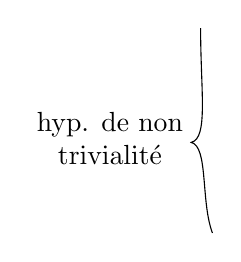
\begin{tikzpicture}[x=1cm,y=1cm]
\draw (0,2.6) .. controls (0,1.8) and (.1,1.2) .. (-.12,1.15) .. controls (.1,1.1) and (0,.4) .. (.15,0);
\node[left] at (-.1,1.2) {\shortstack{hyp. de non\\trivialité}};
\end{tikzpicture}}}
4°) Pour tte $\omega\in\unsure{\Gamma|\Omega}(X)$, l'hom correspondant
\[
\diagram{\begin{tikzcd}
\rho_{Y/X} \arrow[r] & \Omega_Y
\end{tikzcd}}
\]
est injectif [deux rives différentes définissent des orientations différentes de Y]

5°) Pour tout $X\in\operatorname{Ob}\mathcal V$, $\Omega(X)\to X$ est surjectif (il existe localement des orientations $\unsure{\omega|\varphi}$ de X; ou encore:
$\forall n\geq1$, $\Omega(\mathbb R^n)$ est non vide)

\margin{\figure{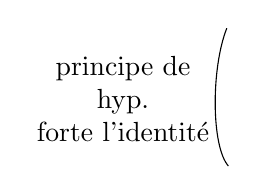
\begin{tikzpicture}[x=1cm,y=1cm]
\draw (.1,1.9) .. controls (-.1,1.4) and (-.1,.4) .. (.12,.15);
\node[left] at (0,1) {\shortstack{\inserted{principe de}\\\deleted{\unsure{hyp.}}\\\deleted{\unsure{forte}} \unsure{l'identité}}};
\end{tikzpicture}}}
6°) Pour tt $X\in\operatorname{Ob}\mathcal V$, $\Omega(X)$ interprété comme espace étalé sur X est séparé sur X, ou encore:
une orientation d'un $X\in\operatorname{Ob}\mathcal V$ est connue en un pt quand on la connaît en des pts arbitrairement voisins. (Il suffit de l'exiger pour $\mathbb R^n$, $n\geq1$, en fait, il sera vrai a posteriori qu'une orientation de $\mathbb R^n$, \inserted{ou de tt X connexe,} est connue quand on le connaît en un seul point\ldots)

\margin{32}
\scanpage{34}
\mspage{5}
(iii) \uline{The} \uline{space} $Y$ \uline{can} \uline{be} \uline{written} \uline{as} \uline{a} \uline{direct} \uline{sum}
\[
Y=Y_1\oplus Y_0,
\]
\uline{where}
\[
\begin{aligned}
Y_1&=\{y\in Y:y\text{ is a T-fixed point}\}\\
&=\theta(Y)
\end{aligned}
\]
\uline{and}
\[
\begin{aligned}
Y_0&=\{y\in Y:0\in\unsure{\mathcal O|O}(y)\}\\
&=\text{kernel of }\theta.
\end{aligned}
\]

PROOF. The assumption that each $\unsure{\mathcal O|O}(y)$ is weakly compact insures that the weak operator closure $S$ of $T$ in $B(Y)$ is compact in the weak operator topology. Moreover, $\unsure{\mathcal O|O}(y)=\{s(y):s\in S\}$ for every $y$ in $Y$. By the lemma, $T$ converges in the weak operator topology to a zero $\theta$ for $S$. Since $t\circ\theta=\theta$ for all $t$ in $T$, $\theta(y)$ is T-fixed for any $y$. If $z$ is any T-fixed point in $\unsure{\mathcal O|\theta}(y)$, then $z=s(y)$ for some $s$ in $S$ and
\[
z=\theta(z)=\theta(s(y))=\theta(y).
\]
\margin{\unsure{;}}

Hence (i) and the first part of statement (ii) hold; (iii) follows trivially. It remains only to show that $T$ converges to $\theta$ in the strong operator topology.
\margin{33}
\scanpage{36}
\[
g=\exp f\qquad f'=\varphi=\unsure{\psi|\Psi}^{1/2}
\]
\[
g'=(\exp f)f'\deleted{=\unsure{(\exp f)\varphi}}
\]
\[
g''=(\exp f)f'^2+(\exp f)f''=(\exp f)(f'^2+f'')
\]
\[
\begin{aligned}
g'''&=(\exp f)f'(f'^2+f'')+(\exp f)(2f'f''+f''')\\
&=(\exp f)(f'^3+3f'f''+f''')
\end{aligned}
\]
\[
\frac{g'''}{g'}=f'^2+3f''+\frac{f'''}{f'}
\]
\[
\frac{g''}{g'}=f'+\frac{f''}{f'}\qquad
\left(\frac{g''}{g'}\right)^2=f'^2+\left(\frac{f''}{f'}\right)^2+2f''
\]
\[
\begin{aligned}
-2\frac{g'''}{g'}+3\left(\frac{g''}{g'}\right)^2
&=\uline{-2f'^2}-\deleted{6f''}-2\frac{f'''}{f'}\\
&\quad+\uline{3f'^2}+3\left(\frac{f''}{f'}\right)^2+\deleted{6f''}\\
&=-2\frac{f'''}{f'}+3\left(\frac{f''}{f'}\right)^2+\deleted{\unsure{3}}f'^2
\end{aligned}
\]
\[
G(t,\exp f)=G(t,f)+3(df)^2
\]
\[
\begin{array}{c}
\Vert\\
-c_t+c_{\exp f}=-c_t+c_f+3(df)^2
\end{array}
\]
\[
\boxed{c_{\exp f}=c_f+\deleted{\unsure{3}}df^2}
\]
\[
c_{\exp f}=c_f+\deleted{\unsure{3}}df^2=c_f+\omega^{\unsure{\otimes2|2}}.
\]
\[
\begin{array}{l}
\varphi=\exp t\\
\varphi'=\exp t\\
\varphi''=\exp t\\
\varphi^{\unsure{'''}}=\exp t
\end{array}
\qquad
\left(-2\frac{\varphi'''}{\varphi'}+3\left(\frac{\varphi''}{\varphi'}\right)^2\right)dt^2=dt^2
\]
\[
c_f+\unsure{\omega^2|\infty}
\]

\margin{\figure{\begin{tikzpicture}[x=1cm,y=1cm]
\node (formula) at (0,1.2) {$\deleted{\unsure{C}}G(z,f)\deleted{\unsure{d}}=\left(-\unsure{2}\frac{f'''}{f'}+3\left(\frac{f''}{f'}\right)^2\right)dz^2$};
\node (note) at (-2,-.2) {\shortstack{\unsure{invariant} \unsure{pour} $\pi$\\\deleted{\unsure{automorphismes|homomorphismes}}\\\unsure{hyperboliques}}};
\draw (-4,.45) .. controls (-4.6,-.25) and (-3.8,-.9) .. (-2.1,-.85) .. controls (-.2,-.9) and (.3,.35) .. (-1,.45) -- cycle;
\draw[->] (-3.6,.45) .. controls (-3.2,.6) and (-3.1,.8) .. (-3.1,1);
\draw (-.8,.8) .. controls (-.4,.55) and (2,.65) .. (2.6,.75);
\node at (2,-.1) {$\dfrac{df}{dz}$};
\node[right] at (2.7,-.1) {\shortstack{forme inv. par\\$\pi$}};
\end{tikzpicture}}}

\margin{$G(f,z)\deleted{\unsure{df^2}}=0$}
\margin{\figure{\begin{tikzpicture}
\node at (0,0) {$\dfrac{d^3z}{df^3}$};
\draw (.4,.05) .. controls (.65,.12) and (1.4,.1) .. (1.7,.05);
\end{tikzpicture}}}
\margin{$G(f,z)=0$}
\margin{$G(z,f)=$}
\margin{$\begin{array}{c}
\unsure{\gamma}.G(z,f)\\
\Vert\\
G(\unsure{\gamma}.z,\unsure{\gamma}.f)\\
\Vert\\
G(\unsure{\gamma}z,f)\\
\Vert\\
G(z,f)
\end{array}$}
\figure{\begin{tikzpicture}\draw (0,0)--(0,1.4);\draw (.17,.05)--(.17,1.3);\end{tikzpicture}}
\margin{35}
\scanpage{37}
$\underline{\overline{\mathrm V}}$\qquad Programme de la Théorie

(Cristaux)
\margin{36}
\scanpage{38}
\margin{\figure{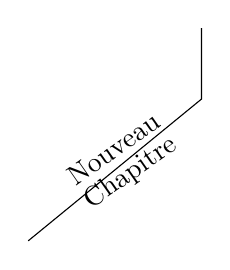
\begin{tikzpicture}\node[rotate=35] at (0,0) {\shortstack{Nouveau\\Chapitre}};\draw (-1.2,-1)--(1,.8)--(1,1.7);\end{tikzpicture}}}
1) Programme de la théorie de Dieudonné sur une base \inserted{$S$} où p est localement nilpotent.

 a) \uline{Foncteur de Dieudonné}. On \deleted{va} définiraun foncteur
\[
\diagram{\begin{tikzcd}
\underline D^*:\quad \mathrm{BT}(S)^0 \arrow[r] & \mathrm{Crisloclib}(S),
\end{tikzcd}}
\]
\margin{$\unsure{\mathbb D|D}^*$}
compatible aux images inverses (donc foncteur cartésien sur la catégorie fibrée des groupes de BT sur des bases où p est \unsure{loc.} nilp.). Si $S_0=\operatorname{Var}(p)$ on a une équivalence de catégories (cf.\qquad plus haut)
\[
\mathrm{Crisloclib}(S)\unsure{\approxeq|\simeq}\mathrm{Crisloclib}(S_0)
\]
de sorte que la donnée de $\underline D^*$ équivaut à la donnée de
\[
\diagram{\begin{tikzcd}
\underline D^*:\quad\mathrm{BT}(S_0)^0 \arrow[r] & \mathrm{Crisloclib}(S_0),
\end{tikzcd}}
\]
i.e. on est ramené \deleted{à la car. p.} au cas S de car. p. \deleted{\unsure{Pour connaitre, d}}
Dans le cas général, $\underline D^*(G)$ ne dépend que de $\deleted{\unsure{D^*}}G_0=G\times_S S_0$.

\deleted{\unsure{Utilis}} Plaçons nous sur $S_0$ de car. p. Utilisant $\underline f_G$ et $\underline V_G$ et la compatibilité de $\underline D^*$ aux images inverses, on voit que \deleted{le foncteur}
$\underline D^*(G_0)$ \deleted{peut}\inserted{$=M$} est naturellement muni de morphismes $F_M,V_M$ \deleted{satisfaisant}
\[
\diagram{\begin{tikzcd}
M^{(p)}=\underline f_S^*(M) \arrow[r,shift left,"F_M"] & M \arrow[l,shift left,"V_M"]
\end{tikzcd}}
\]
satisfaisant
\[
V_MF_M=p\operatorname{id}_M,\quad F_MV_M=p\operatorname{id}_{\unsure{M}}(p).
\]
On appelle un tel triple $(M,F_M,V_M)$ un (F-V-\uline{cristal}\inserted{ ou \uline{cristal de Dieudonné}}), et on a donc un foncteur
\[
\diagram{\begin{tikzcd}
\underline D^*:\quad\mathrm{BT}(S_0) \arrow[r] & \text{F-V-Cris}(S_0).
\end{tikzcd}}
\]
C'est ce foncteur qui mérite le nom de \uline{foncteur de Dieudonné}. On \deleted{\unsure{pouve|prouve}} \deleted{prouve que} voit que sa formation commute à tout changement de\inserted{ }base. De plus, on prouve que pour $S_0$ spectre d'un corps parfait, il coïncide \deleted{avec} à isomorphisme canonique près avec le foncteur de Dieudonné habituel, qui est alors une équivalence de catégories, de sorte que dans ce cas la
\margin{37}
\scanpage{39}
connaissance de $\underline D^*(G_0)$ permet de reconstituer $G_0$. Ainsi, dans le cas général, la connaissance de $\underline D^*(G_0)=M$ comme F-V-cristal sur $S_0$ permet de retrouver les fibres de $G_0$ en des corps parfaits au dessus de $S_0$; cela justifie donc le sentiment que pour l'essentiel, on a saisi avec le cristal $M=\underline D^*(G_0)$ la famille des $G_{0\bar s}$. Une question importante \inserted{\unsure{en ce sens}} que je n'ai pas résolue est :

\uline{Problème} 1 : Le foncteur de Dieudonné sur une base $S_0$ de car. p est-il pleinement fidèle ? \deleted{Quel est}\deleted{\inserted{\unsure{la|le}}} Son image essentielle est-elle formée des F-V-cristaux ``admissibles'' définis plus bas ?

Pour résoudre cette question, il me semble qu'il faudrait arriver à formuler une théorie de Dieudonné sur \deleted{des bases de car. p} $S_0$ pour des schémas en \inserted{p-}groupes finis localement libres sur $S_0$ quelconques, ou du moins pour ceux plats sur un $\Lambda_n$, en trouvant une équivalence entre \deleted{entre} la catégorie de\deleted{s} ces groupes sur $S_0$, et une catégorie de F-V-cristaux sur $S_0$ \uline{muni de} \figure{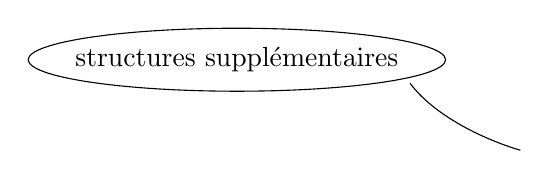
\begin{tikzpicture}[baseline=(s.base)]
\node[inner sep=1pt] (s) at (0,0) {\uline{structures supplémentaires}};
\draw (0,0) ellipse (2.65cm and .4cm);
\draw (2.2,-.3) .. controls (2.5,-.7) and (3.1,-1) .. (3.6,-1.15);
\end{tikzpicture}}\inserted{$(\unsure{*|\dagger})$} que je n'ai pas réussi à dégager encore, et qui très probablement impliqueront la donnée d'une \uline{filtration} sur un objet \inserted{convenable} d'une catégorie dérivée \ldots
\margin{sans doute inutile si $\unsure{S_0}$ est parfait}
\margin{38}
\scanpage{40}
\uline{Problème} 2. Développer une telle théorie de Dieudonné pour des p-Grou-\linebreak
pes finis localement libres sur une base $S_0$ de car.p 0. Si $S_0$ est parfait
établir une \inserted{anti-}équivalence entre la catégorie des Groupes finis localement libres sur $S_0$ qui sont \uline{plats sur} $\Lambda_n=\underline Z/p_{\deleted{\unsure{n}}}^{\inserted{n}}\underline Z$ (cf.\qquad), et la catégorie des $\underline W_n(\underline O_S)$-Modules localement libres M, muni de $F_M$ et $V_M$ \deleted{comme \unsure{d'habi}} satisfaisant les conditions habituelles.

Une solution affirmative à ce dernier problème devrait évidemment impliquer une solution affirmative au problème 1 dans le cas où $S_0$est un schéma \uline{parfait}.
\margin{39}
\scanpage{41}
b) \uline{Filtration}s\deleted{\unsure{ass}} \uline{associées aux cristaux de Dieudonné}. Revenons au cas d'un S général (sur lequel p soit loc. nilp.). On \unsure{définita|définira} alors, pour tout $G\in\operatorname{Ob}\mathrm{BT}(S)$, une filtration \deleted{en deux crans} de MoDule localement libre $\underline D^*(G)_S$ sur S par un sous-Module localement facteur direct (donc localement libre de t.f.) \inserted{$\uline{Fil}^{1}=$} $\underline\omega_G$, donnant lieu à une suite exacte
\[
(*)\qquad
\diagram{\begin{tikzcd}
0 \arrow[r] & \underline\omega_G \arrow[r] & \underline D^*(G) \arrow[r] & \underline t_{G^*} \arrow[r] & 0,
\end{tikzcd}}
\]
où en fait $\underline\omega_G$ est le module des différentielles invariantes sur le groupe formel $\overline G\subset G$ associé à G (qui sera construit plus bas), et $\underline t_G=\underline\omega_{G^*}^{\vee}$ est l'Algèbre de Lie associée au groupe de BT dual $G^*$ de G (définition à reporter aux généralités sur les goupes de BT). Cette \deleted{\unsure{filtr}} suite exacte est fonctorielle \inserted{en G} et compatible aux images inverses par un $S'\longrightarrow S$.

\margin{(*) \unsure{formule inutile si} $S_0$ \unsure{parfait}}
\margin{40}
\scanpage{42}
Appelons F-V-\uline{\unsure{cristal}} \uline{filtré}\inserted{ \uline{sur} S} (par abus de langage) un F-V-cristal en Mod. loc. lib. sur S muni de\deleted{une filtr} la donnée d'une filtration de $M_S$ par une sous-module localement facteur direct. On trouve donc en fait un foncteur
\[
\diagram{\begin{tikzcd}
\mathrm{BT}(S) \arrow[r] & \text{F-V-cris fil }(S),
\end{tikzcd}}
\]
compatible aux images inverses.

\inserted{\uline{Remarque}}
La filtration (*) doit être considérée comme étant l'équivalent d'une filtration ``de Hodge'' sur une \unsure{cohomoologie|cohomologie} de De Rham \inserted{relative} en dimension 1. \deleted{Pour expliciter} Ce point\deleted{, partons par exemple \unsure{d'un schéma abélien} A sur S, et prenons $G=\unsure{A}(\infty)=\unsure{\lim|\varinjlim}A(n)$. On peut alors}\inserted{ sera explicité plus bas.}

Soit maintenant S' un épaississement à p.div. de S. On se propose de trouver tous les prolongements possibles (à isom. près) \unsure{da|du} groupe de BT G donné sur S en un groupe de BT G' sur S'. On \deleted{trouve} prouvera que si à tout tel G', on associe la filtration correspondante de $D(G')_{S'}=\underline D^*(G)_{S'}=\underline D^*(G_0)_{S'}$ (cf.\qquad pour le fait que S' peut être envisagé comme un objet du site cristallin absolu de $S_0$), qui prolonge la filtration qu'on a sur $\underline D^*(G)_S=\underline D^*(G_0)_S=\underline D^*(G')|S$, on trouve une bijection entre l'ensemble des classes d'isomorphie cherchés et l'ensemble des filtrations qui prolongent. De façon plus précise, on a:\deleted{une équivalence de catégories}

\margin{\figure{\begin{tikzpicture}\draw (0,0)--(0,1.5);\end{tikzpicture}}}
\uline{Théorème de déformation pour les groupes de} BT : Soient S un schéma où p est loc. nilp., S' un épaississement à p.div. de S, Considérons le foncteur canonique
\[
\diagram{\begin{tikzcd}[column sep=large]
\mathrm{BT}(S') \arrow[r] & \begin{array}{l}
\text{catégorie des }\deleted{\text{triples}}\inserted{\text{paires}}\text{ d'un groupe de BT G sur S, et}\\
\text{d'un}\deleted{\text{e}}\text{ sous-module localement facteur direct de}\\
\underline D^*(G)_{S'}\text{ qui prolonge le sous-module }\operatorname{Fil}^1\underline D^*(G)_S=\underline\omega_G\\
\text{de }\underline D^*(G)_S.
\end{array}
\end{tikzcd}}
\]
\margin{\figure{\begin{tikzpicture}\draw (0,0)--(0,.6);\end{tikzpicture}}}
Ce foncteur est une \uline{équivalence de catégories}, \inserted{\uline{si} S' \uline{est à p. div. nil} ou si on se borne à des G qui sont infinitésimaux, ou à \unsure{duaux} infinitésimaux.}
\figure{\begin{tikzpicture}\draw (0,.1)..controls (3,.45) and (5,-.15)..(7,.1)--(13,.1);\end{tikzpicture}}

\inserted{Remarques}
Si le \deleted{\unsure{questio|question}} problème 1 avait une réponse affirmative, on en conclurait une description de la catégorie des groupes de BT sur S en termes de cristaux de Dieudonné filtrés sur S, en appliquant le théorème de
\margin{41}
\scanpage{43}
déformation aux cas du couple $(S_0,S)$, \deleted{\unsure{en}} notant que l'idéal $p\underline O_S$ est bien un idéal à puissances divisées. On notera d'ailleurs que le théorème de déformations dans le cas \deleted{envisagé} général $(S,S')$ envisagé dans son énoncé est en fait équivalent au cas particulier d'un couple $(S_0,S)$, comme il est formel via $\mathrm{Crisloclib}(S)\xrightarrow{\approx}\mathrm{Crisloclib}(S_0)$.

\inserted{\uline{Problème} 3\quad Trouver variante du th. de déformation p\textsuperscript{r} les p-Groupes}
\margin{\figure{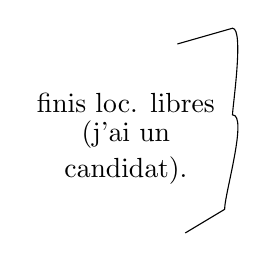
\begin{tikzpicture}
\node[left] at (-.1,0) {\shortstack{finis loc. libres\\(j'ai un\\candidat).}};
\draw (-.7,1.2)--(0,1.4)..controls (.15,1.4) and (0,.4)..(0,.3)..controls (.2,.3) and (-.1,-.7)..(-.1,-.9)--(-.6,-1.2);
\end{tikzpicture}}}

c) F-V-\uline{cristaux admissibles en car.} p. Revenons au cas d'un schéma de car. p. Le cristal de Dieudonné $D^*(G_0)$ étant muni d'une filtration canonique (de $D^*(G_0)_{S_0}$), on pourrait craindre que le problème 1 est mal posé, et qu'il faudrait envisager le foncteur comme étant à valeurs dans des cristaux de Dieudonné filtrés. En fait, dans le cas envisagé ici, il se trouve que la filtration est uniquement déterminée en \unsure{ytermes|termes} de la structure de cristal de Dieudonné, comme on va l'expliquer maintenant.

Considérons le morphisme de topos annelés (qui aura été défini déjà précédemment, dans le par. d'exemples de cristaux, pour les relations entre cristaux et vecteurs de Witt)
\[
\diagram{\begin{tikzcd}
\phi:\quad S_{0\,\unsure{\mathrm{cris}|\mathrm{crys}}/\underline F_p} \arrow[r] & S_0 \arrow[l,bend right=55,"\varepsilon"'] .
\end{tikzcd}}
\]
Soit $M=D^*(G_0)$, et soit $M_0$ sa restriction au site cristallin rel. à $\underline F_p$. Il se trouve que \deleted{la suite} d'après $FV=p$, $VF=p$, les composés dans la suite
\[
\diagram{\begin{tikzcd}
\unsure{M}_0^{(p)} \arrow[r,"F_{M_0}"] & M_0 \arrow[r,"V_{M_0}"] & M_0^{(p)} \arrow[r,"F_{M_0}"] & M_0
\end{tikzcd}}
\]
sont nuls; en fait, on prouvera mieux, à savoir que \inserted{pour tout cristal de Dieud. M,} la suite précédente est exacte (terme à terme sur tout épaississement à p.div. de car.p de $S_0$) et on obtient ainsi des sous-cristaux en modules loc. libres
\[
\operatorname{Ker}V_{M_0}=\operatorname{Im}F_{M_0}\subset M_0,\quad
\operatorname{Ker}F_{M_0}=\operatorname{Im}V_{M_0}\subset M_0^{(p)}.
\]
Ceci dit, \deleted{le sous-Module $\operatorname{Fil}^1$} notons que $M_{S_0}=\varepsilon^*(M_0)$, donc
\[
\phi^*(M_{S_0})\simeq M_0^{(p)}
\]
donc on a
\[
\phi^*(\operatorname{Fil}^1(M_{S_0}))\subset M_0^{(p)}.
\]
Ceci posé, on montre qu'on a
\margin{42}
\scanpage{44}
\[
\phi^*(\mathrm{Fil}^1(M_{S_0}))=\operatorname{Ker}F_{M_0}
(=\operatorname{Im}V_{M_0})\subset M_0^{(p)}.
\]
D'autre part, on montre que $\phi$ a des propriétés de fidélité telles que la relation précédente détermine sans ambiguité le sous-Module localement facteur direct $\mathrm{Fil}^1$ de $M_{S_0}$.

On dira qu'un \inserted{F-V-}cristal en modules loc. lib. $M_0$ sur le site cristallin de $S_0$ au dessus de $\underline{\mathrm F}_p$ est \uline{admissible} s'il existe un sous-module loc. \deleted{\unsure{facteur}} facteur direct $\mathrm{Fil}^1$ de $\unsure{M_{0S}}$ tel que l'on ait la relation précédente; \deleted{On}
\inserted{$\mathrm{Fil}^1$ est unique et \deleted{\unsure{déterm}}\figure{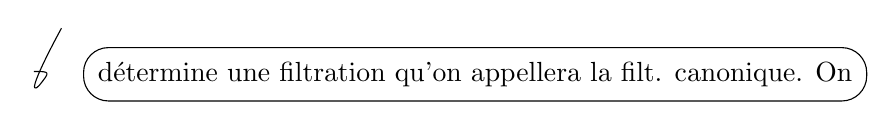
\begin{tikzpicture}
\node[inner sep=5pt] (t) {détermine une filtration qu'on appellera la \uline{filt.} \uline{canonique}. On};
\draw[rounded corners=9pt] (t.north west) -- (t.north east) -- (t.south east) -- (t.south west) -- cycle;
\draw ([xshift=-8pt,yshift=7pt]t.north west) .. controls ([xshift=-17pt]t.west) and ([xshift=-20pt,yshift=-8pt]t.west) .. ([xshift=-16pt,yshift=-4pt]t.west) .. controls ([xshift=-12pt,yshift=1pt]t.west) .. ([xshift=-18pt,yshift=1pt]t.west);
\end{tikzpicture}}}
dit de même qu'un \unsure{Cristal|cristal} de Dieudonné \inserted{$M$} sur $S_0$ est admissible si sa restriction $M_0$ \deleted{sur} au site cristallin rel. à $\underline{\mathrm F}_p$ est admissible. On voit donc que si $M$ est le cristal de Dieudonné associé à un groupe de BT sur $S_0$, $M$ est admissible, et la filtration de $M_{S_0}$ envisagée dans b) est la filtration canonique définie précédemment.

\margin{d) Passage à la limite : \unsure{pour des|pour un} \unsure{anneaux|anneau} $A$ \unsure{séparés|séparé} et \unsure{complets|complet} pour \unsure{top.} p-adique}
\figure{\begin{tikzpicture}[x=1cm,y=1cm]
\draw (0,2.3) .. controls (.8,2.6) and (.2,.7) .. (.75,.45) .. controls (.9,.35) and (1.05,.25) .. (1.3,.25);
\draw (1.3,.25) .. controls (.6,.25) and (.65,-.1) .. (.25,-.4) .. controls (-.3,-.9) and (-1.1,-1.15) .. (-2,-1.35);
\end{tikzpicture}}
\margin{e) Théorie : isogénies \uline{et} \unsure{th.} de Tate}
\margin{f) Dualité}

2) \uline{Théorie de déformations pour les schémas abéliens.}

\inserted{a)} Dans cette théorie, il n'y a plus de nombre premier privilégié, par contre il faut travailler avec le site cristallin \uline{nilpotent}. On trouve un foncteur \inserted{contravariant} de la catégorie des schémas abéliens sur le schéma $S$ vers les \deleted{sites} cristaux sur le site cristallin nilpotent de $S$
\[
\text{Schémab}(S)\longrightarrow\mathrm{Crisloclib}_{\mathrm{nilp}}(S)
\]
qui peut être défini par exemple comme
\[
\inserted{(*)}\qquad \underline{\mathbb D}^{*}:A\longmapsto R^1f_{A\mathrm{cris}*}
(\deleted{\unsure{A}}\inserted{\unsure{\mathcal O}_{A\mathrm{cris}}})
\]
où on considère
\[
f_{\mathrm{cris}}:A_{\mathrm{crisnilp}}\longrightarrow S_{\mathrm{crisnilp}}
\]
induit par $S$. Par une variante du théorème de changement de base, on voit que
\[
\mathbb D^*(A)_S=\deleted{\unsure{R^1f_{A*}}}\underline{\mathrm H}^1_{\mathrm{DR}}(A/S)
\overset{\mathrm{dfn}}=R^1f_{A*}(\Omega^\bullet_{A/S}).
\]
Pour calculer $\mathbb D^*(A)_{S'}$, $S'$ épaississement à p.div. loc. nilpotentes de $S$, on aura pour tout prolongement \deleted{canonique} de $A$ en un schéma abélien $A'$ sur $S'$
\margin{43}
\scanpage{45}
\[
\mathbb D^*(A)_{S'}=\deleted{R^1f}\underline{\mathrm H}^1_{\mathrm{DR}}(A'/S')\quad\deleted{\unsure{*}}.
\]
On notera que d'après un théorème connu (cf. livre de Mumford Geometric Invariant theory) il existe toujours un $A'$ pour $S$ affine; le fait que \deleted{\unsure{A}}\inserted{$\mathrm H^1(A'/S')$} ne dépende, à isomorphisme près, pas du prolongement choisi de $A$, peut être considéré ici comme conséquence du tapis de la cohomologie cristalline.

En fait, utilisant la filtration de \deleted{De Rham}\inserted{Hodge} sur la cohomologie de De Rham, on trouve une filtration sur $\mathbb D^*(A)_{\unsure{S|S'}}$, savoir
\[
0\longrightarrow R^0f_*(\underline\Omega^1_{A/S})\longrightarrow
\underline{\mathrm H}^1_{\mathrm{DR}}(A/S)\longrightarrow R^1f_*(\underline{\mathrm O}_S)\longrightarrow0,
\]
qu'on peut interpréter comme
\diagram{\begin{tikzcd}[column sep=small]
(**) & 0\arrow[r] & \underline t_A^\vee\arrow[r]\arrow[d,equal] & \mathbb D^*(A)_S\arrow[r] & \underline t_{A^*}\arrow[r] & 0 & \unsure{-}.\\
&&\underline\omega_A
\end{tikzcd}}

Le foncteur $(*)$ et la suite exacte $(**)$ sont fonctoriels en $A$ et \unsure{compatibles} avec image inverse. On peut \deleted{envisager} considérer que le foncteur $(*)$ se factorise en
\[
\mathbb D^*:\text{Schémab}(S)\longrightarrow\mathrm{Crisloclib}_{\mathrm{nilp}}\mathrm{fil}(S)
\]
vers les cristaux en modules localement libres ``filtrés''(en deux crans localement libres). Utilisant cette factorisation, on trouve que pour un objet $S'$ du site cristallin nilpotent de $S$, la donnée d'un prolongement de $A$ en un schéma \inserted{abélien} $A'$ sur $S'$ revient à la donnée d'un prolongement de la filtration canonique $(**)$ de $D^*(A)_S$ en une filtration (à quotients localement libres) de $D^*(A)_{S'}$. Plus précisément, on a le

\uline{Théorème de déformation pour les schémas abéliens}. Soient $S$ un schéma, $S'$ un voisinage à puissances div. loc. nilp. de $S$, alors le foncteur naturel
\diagram{\begin{tikzcd}[column sep=small]
\text{Schémab}(S')\arrow[r] & \begin{gathered}
\text{catégorie des couples }(A,\deleted{\unsure{\Phi}}\,\unsure{\mathrm{Fil}}^1)\text{ d'un schéma abélien}\\
A\text{ sur }S\text{ et d'un sous-module localement facteur direct}\\
\mathrm{Fil}^1\ \inserted{\text{de }\mathbb D^*(A)_{S'}}\text{ prolongeant }\mathrm{Fil}^1\mathbb D^*(A)_S\simeq\underline\omega_A
\end{gathered}
\end{tikzcd}}
est une équivalence de catégories.

\inserted{b)} On peut donner une deuxième interprétation du foncteur $\unsure{\mathbb D|D}^*$ sur les
\margin{44}
\scanpage{46}
schémas abéliens, \inserted{permettant de définir un foncteur qu.inverse du foncteur du théorème.} Pour ceci, on considère pour tout schéma abélien $A$ sur $S$ son extension vectorielle universelle, qui est une extension
\[
0\longrightarrow\underline t_{A^*}^{\vee}\;-\;E(A)\;-\;A\longrightarrow0.
\]
Il se trouve qu'on peut trouver un cristal en groupes lisses canonique sur $S$, soit $\underline E(\unsure{A})$, tel que l'on ait
\[
E(A)\unsure{\simeq|\cong}\underline E(A)_S.
\]
La définition est telle que \deleted{pour tout le foncteur}\inserted{$A$} $\underline E(A)$ définisse un foncteur
\[
\text{Schémab}(S)\longrightarrow\text{Cris Groupes lisses}_{\mathrm{nilp}}(S)
\]
compatible aux changements de base, l'isomorphisme précédent étant également fonctoriel et compatible aux changements de base. Il s'ensuit donc que l'on peut définir $\underline E(A)_{\deleted{S}}$ comme $S'\mapsto\underline E(A)_{S'}$, avec
\[
\underline E(A)_{S'}=E(A'),
\]
$A'$ désignant un schéma abélien qui prolonge $A$ sur $S'$, \deleted{\unsure{à}} à charge de définir \deleted{un}\inserted{un système transitif d'} isomorphismes canoniques entre les groupes obtenus pour des prolongements différents. Dans le cas où $S$ est de \unsure{caractééristique|caractéristique} nulle (donc plus question de puissances divisées !) cela est particulièrement simple; on prouve qu'il existe à isomorphisme \uline{unique} près un seul schéma en groupes lisses $E'$ sur l'épaississement $S'$ de $S$ qui prolonge $E$ (NB il suffirait même d'un nilépaississement, comme on voit par passage à la limite à partir du cas noethérien): c'est le résultat déjà signalé dans ma vieille lettre à Tate. Dans le cas général, c'est plus délicat, et peut se faire par ``la méthode de l'exponentielle'', qui sera exposée dans le contexte analogue des groupes de BT dans la suite du séminaire. On peut aussi définir $\underline E(A^*)$ par
\[
\underline E(A^*)=R^1f_{A\mathrm{cris}*}(\underline G_{m\,A_{\mathrm{cris}}}),
\]
où $A_{\mathrm{cris}}$ désigne le topos cristallin \deleted{\unsure{abso}} nilpotent absolu (relativement à $\underline Z$ ): cette méthode peut également s'adapter au cas des groupes de BT.

Quoi qu'il en soit de la méthode utilisée pour définir $\underline E(A)$, on
\margin{45}
